\documentclass{beamer}
\usetheme{Madrid}
\usecolortheme{whale}

% Package imports
\usepackage{tikz}
\usepackage{listings}
\usepackage{xcolor}

% Custom colors
\definecolor{customblue}{RGB}{48, 52, 159}

% Title page info
\title{Research Plan for CSE3000 Research Project}
\author{Vladimir Sachkov}
\date{November 21, 2024}

\lstdefinestyle{customcode}{
    basicstyle=\tiny\ttfamily,
    keywordstyle=\color{blue},
    commentstyle=\color{green!60!black},
    stringstyle=\color{purple},
    numbers=left,
    numberstyle=\tiny,
    numbersep=5pt,
    frame=single,
    breaklines=true,
    showstringspaces=false,
    columns=fullflexible,
    backgroundcolor=\color{gray!10},
    keywords={def, while, return, pass}
}

\begin{document}

% Title frame
\begin{frame}
    \titlepage
\end{frame}

% Research Questions frame
\begin{frame}
    \frametitle{Research Questions}
    
    \begin{center}
        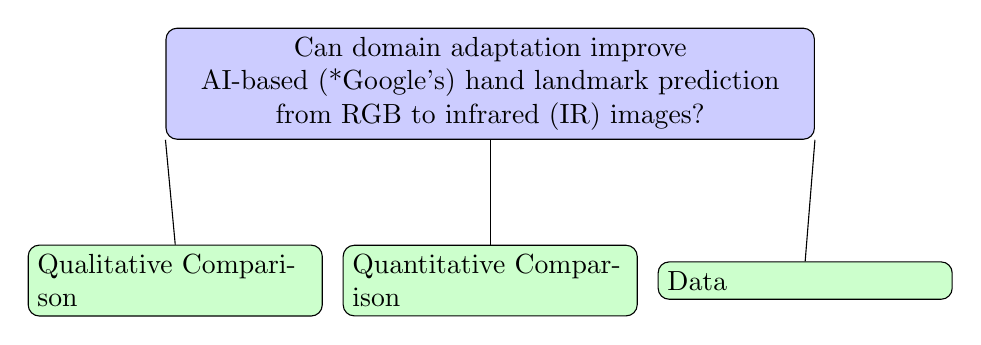
\begin{tikzpicture}
            % Main question box
            \node[draw, rounded corners, fill=blue!20, text width=8cm, align=center] 
                (main) at (0,2) {Can domain adaptation improve\\AI-based (*Google's) hand landmark prediction\\from RGB to infrared (IR) images?};
            
            % Connected concepts - adjusted positions and widths
            \node[draw, rounded corners, fill=green!20, text width=3.5cm] 
                (qual) at (-4,-0.5) {Qualitative Comparison};
            \node[draw, rounded corners, fill=green!20, text width=3.5cm] 
                (quant) at (0,-0.5) {Quantitative Comparison};
            \node[draw, rounded corners, fill=green!20, text width=3.5cm] 
                (data) at (4,-0.5) {Data};
            
            % Draw lines connecting nodes from bottom of main box to top of category boxes
            \draw[-] (main.south west) -- (qual.north);
            \draw[-] (main.south) -- (quant.north);
            \draw[-] (main.south east) -- (data.north);
        \end{tikzpicture}
    \end{center}
    
    \begin{columns}[T] % Added [T] for top alignment
        \column{0.33\textwidth}
        \textbf{Qualitative Comparison}
        \begin{itemize}
            \item Availability of data
            \item Shallow vs Deep models
            \item Scalability
        \end{itemize}
        
        \column{0.33\textwidth}
        \textbf{Quantitative Comparison}
        \begin{itemize}
            \item Comparative metrics
            \item Real-time inference maintenance
        \end{itemize}
        
        \column{0.33\textwidth}
        \textbf{Data}
        \begin{itemize}
            \item Data augmentation
            \item Google's model limitations
        \end{itemize}
    \end{columns}
\end{frame}

% Methodology frame
\begin{frame}[fragile]
    \frametitle{Methodology (1/2): Setup and Core Components}
    \lstset{style=customcode}
    \begin{lstlisting}
# 1. Data Collection and Initial Setup
DATA = Upload_and_clean_infrared_videos()
DETECTOR = GoogleMediaPipe.HandLandmarkDetector()

# 2. Domain Adaptation Methods to Explore
ADAPTATION_METHODS = [
    "Feature Alignment",        # Start with simpler approach
    "Adaptive Batch Norm",      # Gradually increase complexity
    "DANN",                     # Deep adversarial learning
    "Correlation Alignment"     # Advanced feature matching
    # And maybe more based on other methods limitations
]

# 3. Core Evaluation Pipeline
def EVALUATE(Data, Detector, Annotations):
    """Measures performance using:
    - Landmark accuracy
    - Inference speed
    - Resource usage"""
    return EvalResults

def DATA_PREP(Data, Method):
    """Prepares data specific to each adaptation method:
    - Data augmentation
    - Feature extraction
    - Domain-specific preprocessing"""
    return (ProcessedData, Annotations)
    \end{lstlisting}
\end{frame}

\begin{frame}[fragile]
    \frametitle{Methodology (2/2): Iterative Research Process}
    \lstset{style=customcode}
    \begin{lstlisting}
# 4. Iterative Experimentation Loop
DEADLINE = datetime(2025, 1, 31)
while datetime.now() < DEADLINE:
    # Phase 1: Setup and Data Preparation
    current_method = select_next_method(ADAPTATION_METHODS)
    prepared_data = DATA_PREP(DATA, current_method)
    
    # Phase 2: Model Adaptation and Testing
    adapted_model = apply_adaptation(DETECTOR, current_method)
    results = EVALUATE(prepared_data, adapted_model)
    
    # Phase 3: Analysis and Improvement
    Reflect(results)

def Reflect(results):
    """Research Documentation and Analysis:
    1. Compare with previous iterations
    2. Document time/resource costs
    3. Identify improvement areas
    4. Plan next adaptation strategy"""
    update_research_findings()
    optimize_pipeline()
    \end{lstlisting}
\end{frame}

% Project Timeline frame
\begin{frame}
    \frametitle{Project Timeline}
    
    \textbf{Key Milestones:}
    \begin{itemize}
        \item \textbf{Nov 2024:} Literature Review \& Evaluation Framework
        \item \textbf{Dec 2024:} Method Implementation \& Midterm Presentation
        \item \textbf{Jan 2025:} Model Optimization \& Comparison Analysis \& Final Documentation
    \end{itemize}
\end{frame}

\end{document}
